\begin{name}
	{\tenchude}
	{TOÁN 10}
	{LỚP TOÁN THẦY PHÁT}
	{Thất bại đơn giản chỉ là cơ hội để ta bắt đầu lại mọi thứ một cách thông minh hơn.}
\end{name}
\Opensolutionfile{ansbook}[ans/ansbookDe2]
\TN
\Opensolutionfile{ans}[ans/ansDe2-TN1]
\begin{ex}%[0D8N1-1]
Lớp bạn An dự định tham gia thi văn nghệ do Đoàn trường triển khai nhân dịp kỷ niệm 26/3. Có $4$ bạn đăng ký tiết mục đơn ca, $2$ nhóm đăng ký tiết mục nhảy hiện đại và $2$ nhóm đăng ký tiết mục hát múa kết hợp. Hỏi lớp bạn An có bao nhiêu cách chọn một tiết mục để dự thi?
\choice
{$16$}
{$256$}
{\True $8$}
{$12$}
\loigiai
{Lớp bạn An có $4+2+2=8$ cách lựa chọn $1$ tiết mục tham gia dự thi.}
\end{ex}

\begin{ex}%[Đề chuẩn hóa Toán 11]%[Nguyễn Trung Kiên]%[0D8N2-3]
Có tất cả bao nhiêu số tự nhiên gồm $3$ chữ số khác nhau được lấy từ các chữ số $1$, $2$, $3$, $4$?
\choice
{$12$}
{\True $24$}
{$4$}
{$3$}
\loigiai{
Số các số tự nhiên gồm $3$ chữ số khác nhau được lấy từ các chữ số $1$, $2$, $3$, $4$ là $\mathrm{A}^3_4=24$.
}
\end{ex}

\begin{ex}%[0D8N3-1]
Trong khai triển $(2x - 5y)^4$ có bao nhiêu số hạng?
\choice
{$6$}
{$4$}
{$7$}
{\True $5$}
\loigiai{
Trong khai triển $(a + b)^{n}$ có $n+1$ số hạng.\\
Như vậy, trong khai triển $(2x - 5y)^4$ có $4 + 1 = 5$ số hạng.
}
\end{ex}

\begin{ex}%[De-chuan-hoa-so-13]%[Huỳnh Quy]%[0D6H1-1]
	Làm tròn số $8316{,}2$ đến hàng chục. Khi đó sai số tuyệt đối của số quy tròn là
	\choice
	{$3{,}6$}
	{$6{,}2$}
	{$3{,}16$}
	{\True $3{,}8$}
	\loigiai{
	Số quy tròn của số $8316{,}2$ đến hàng chục là $8320$.\\
	Do đó sai số tuyệt đối của số quy tròn là $|8320-8316{,}2|=3{,}8$.
	}
\end{ex}

\begin{ex}%[H]%[BG10-3in1, Phạm Ngọc Trung]%[0D6H4-2]
	Cho mẫu số liệu sau
	\begin{center}
		\begin{tabular}{ccccccccc}
			$10$ & $13$ & $15$ & $2$ & $10$ & $19$ & $2$ & $5$ & $7$
		\end{tabular}
	\end{center}
	Giá trị các tứ phân vị của mẫu số liệu sau lần lượt là
	\choice
	{$Q_1=3$, $Q_2=5$, $Q_3=14$}
	{$Q_1=4$, $Q_2=10$, $Q_3=14$}
	{$Q_1=3$, $Q_2=10$, $Q_3=15$}
	{\True $Q_1=3$, $Q_2=10$, $Q_3=14$}
	\loigiai{
		Mẫu số liệu trên được sắp xếp theo thứ tự tăng dần
		\begin{center}
			\begin{tabular}{ccccccccc}
				$2$ & $2$ & $4$ & $7$ & $10$ & $10$ & $13$ & $15$ & $19$
			\end{tabular}
		\end{center}
		Trung vị của mẫu số liệu trên là $10$.\\
		Trung vị của dãy $2$, $2$, $4$, $7$ là $\dfrac{2+4}{2}=3$.\\
		Trung vị của dãy $10$, $13$, $15$, $19$ là $\dfrac{13+15}{2}=14$.\\
		Vậy $Q_1=3$, $Q_2=10$, $Q_3=14$.
	}
\end{ex}

\begin{ex}%[0D0N1-2]
	Gieo con xúc xắc hai lần. Biến cố $A$ là biến cố để sau hai lần gieo có ít nhất một mặt $6$ chấm xuất hiện là
	\choice
	{$A=\{(1;6),(2;6),(3;6),(4;6),(5;6)\}$}
	{$A=\{(1;6),(2;6),(3;6),(4;6),(5;6),(6;6)\}$}
	{\True $A=\{(1;6),(2;6),(3;6),(4;6),(5;6),(6;6),(6;1),(6;2),(6;3),(6;4),(6;5)\}$}
	{$A=\{(1;6),(2;6),(3;6),(4;6),(5;6),(6;1),(6;2),(6;3),(6;4),(6;5)\}$}
	\loigiai{ Gieo con xúc xắc hai lần.\\
		Biến cố $A$ là biến cố để sau hai lần gieo có ít nhất một mặt $6$ chấm xuất hiện là  \[A=\{(1;6),(2;6),(3;6),(4;6),(5;6),(6;6),(6;1),(6;2),(6;3),(6;4),(6;5)\}.\]
	}
\end{ex}

\begin{ex}%[0D0N1-3]
	Gieo một đồng xu liên tiếp hai lần. Số phần tử của biến cố để mặt ngửa xuất hiện đúng $1$ lần là
	\choice
	{\True $2$}
	{$4$}
	{$5$}
	{$6$}
	\loigiai{
		Liệt kê ta có: $A=\{NS;SN\}$.
	}
\end{ex}

\begin{ex}%[0H9N3-1]%[tex hóa đề ck2-form 2025-đợt 2-Hồ Đức Bân]
	Trong mặt phẳng tọa độ $Oxy$, cho đường thẳng $d\colon x-2y+3=0$. Một vectơ pháp tuyến của đường thẳng $d$ là
	\choice
	{\True $\overrightarrow{n}=(1;-2)$}
	{$\overrightarrow{n}=(2;1)$}
	{$\overrightarrow{n}=(-2;3)$}
	{$\overrightarrow{n}=(1;3)$}
	\loigiai{
		Một vectơ pháp tuyến của đường thẳng $d$ là $\overrightarrow{n}=(1;-2)$.
	}
\end{ex}

\begin{ex}
	Phương trình nào sau đây là phương trình tham số của đường thẳng $d$ đi qua điểm $A(1;2)$ và có vectơ chỉ phương $\overrightarrow{u}=(3;4)$ là
	\choice
	{$\heva{&x=1+3t\\&y=2+4t}$}
	{$\heva{&x=1-3t\\&y=2-4t}$}
	{\True $\heva{&x=1+3t\\&y=2-4t}$}
	{$\heva{&x=1-3t\\&y=2+4t}$}
	\loigiai{
		Phương trình tham số của đường thẳng $d$ đi qua điểm $A(1;2)$ và có vectơ chỉ phương $\overrightarrow{u}=(3;4)$ là
		\[\heva{&x=1+3t\\&y=2-4t}.\]
	}
\end{ex}

\begin{ex}%[0H9N3-3]
	Xác định vị trí tương đối của đường thẳng
	$d \colon x-2y+1=0$ và đường thẳng $d' \colon \heva{& x=t\\ & y=3-2t}$.
	\choice
	{Song song}
	{Trùng nhau}
	{\True Vuông góc nhau}
	{Cắt nhau}
	\loigiai{
		Ta có $\vec{n_d} =\vec{u_{d'}}$ nên $d$ và $d'$ vuông góc.
	}
\end{ex}


\begin{ex}%[0H9N5-1]
	Trong mặt phẳng $O x y$, tọa độ các tiêu điểm của elip có phương trình chính tắc $\dfrac{x^2}{25}+\dfrac{y^2}{16}=1$ là
	\choice
	{\True $F_1(-3 ; 0)$; $F_2(3 ; 0)$}
	{$F_1(0 ;-4)$; $F_2(0 ; 4)$}
	{$F_1(-4 ; 0)$; $F_2(4 ; 0)$}
	{$F_1(0 ;-3)$; $F_2(0 ; 3)$}
	\loigiai{ Ta có $\heva{&a^2=25\\&b^2=16}\Rightarrow c^2=a^2-b^2=25-16=9.$\\
		Tọa độ các tiêu điểm của elip là $F_1(-3 ; 0)$; $F_2(3 ; 0)$.
	}
\end{ex}

\begin{ex}%[0H9N5-5]%[Duan15-CKII-HN23-24-Trần Xuân Hòa]%[Chuyen Hùng Vương - Phú Thọ]
	Phương trình nào sau đây là phương trình chính tắc của hypebol?
	\choice
	{\True $\dfrac{x^2}{4}-\dfrac{y^2}{9}=1$}
	{$\dfrac{x^2}{9}+\dfrac{y^2}{4}=1$}
	{$\dfrac{x^2}{4}-\dfrac{y^2}{9}=-1$}
	{$\dfrac{x^2}{9}+\dfrac{y^2}{9}=1$}
	\loigiai{
		Phương trình chính tắc của hypebol là $\dfrac{x^2}{4}-\dfrac{y^2}{9}=1$.
	}
\end{ex}
\Closesolutionfile{ans}

\TNTF
\Opensolutionfile{ans}[ans/ansDe2-TN2]
\begin{ex}%[0D6H4-2]
	Mẫu số liệu thống kê chiều cao (đơn vị: mét) của $10$ cây bạch đàn là:
	\begin{center}
		\begin{tabular}{cccccccccc}
			6,0 & 6,5 & 7,4 & 8,6 & 8,0 & 7,6 & 7,2 & 9,1 & 8,5 & 7,2
		\end{tabular}
	\end{center}
	Các mệnh đề sau \textbf{đúng} hay \textbf{sai}?
	\choiceTF
	{\True Khoảng biến thiên của mẫu số liệu là $3,1$}
	{\True Khoảng tứ phân vị của mẫu số liệu $1,3$}
	{Quy tròn phương sai của mẫu số liệu với độ chính xác $d=0,005$ là $0,85$}
	{\True Sai số tương đối của số quy tròn của phương sai trên xấp xỉ $0,6\%$}
	\loigiai{
		\begin{itemchoice}
			\itemch Chiều cao lớn nhất, nhỏ nhất của cây bạch đàn tương ứng là $9,1; 6,0$. Do đó khoảng biến thiên của mẫu số liệu là $R=9,1-6,0=3,1$.
			\itemch Sử dụng máy tính bỏ túi ta được $Q_1=7,2$, $Q_3=8,5$.\\
			Khoảng tứ phân vị của mẫu số liệu là $\Delta Q=Q_3-Q_1=8,5-7,2=1,3$.
			\itemch Phương sai của mẫu số liệu là $s^2=0,8349$. Quy tròn phương sai với độ chính xác $d=0,005$ là $0,83$.
			\itemch Sai số tương đối của số quy tròn của phương sai trên là
			\[\delta=\dfrac{0,8349-0,83}{0,83}\approx 0,006=0,6\%.\]
		\end{itemchoice}
	}
\end{ex}

\begin{ex}%[0H9H3-2]
	Cho đường thẳng $d$ có phương trình $-2x+y-1=0$.
	\choiceTF
	{Một vectơ chỉ phương của đường thẳng $d$ là $\overrightarrow u_d =\left(-2;1\right)$}
	{\True Điểm $M(1;3)$ thuộc đường thẳng $d$}
	{Đường tròn $(C)$ tâm $I(1;2)$, bán kính $R=\sqrt{5}$ có phương trình là $x^2+y^2-2x-4y+5=0$}
	{\True Đường thẳng $d$ cắt đường tròn $(C)$ tại hai điểm}
	\loigiai{
		\begin{itemchoice}
			\itemch
			Một vectơ chỉ phương của đường thẳng $d$ là $\overrightarrow u_d =\left(1;2\right)$.
			\itemch
			Thay $M(1;3)$ vào phương trình đường thẳng $d$ ta có $-2\cdot 1 +3-1=0$ (luôn đúng).
			\itemch
			Phương trình đường tròn $(C)$ có dạng $(x-1)^2+(y-2)^2=5 \Leftrightarrow x^2+y^2-2x-4y=0$.
			\itemch
			Ta có $\mathrm{d}(I,d)=\dfrac{|-2\cdot 1+2-1|}{\sqrt{(-2)^2+1^2}}=\dfrac{1}{\sqrt{5}}<R$.
			Do đó đường thẳng $d$ cắt đường tròn $(C)$ tại hai điểm.
		\end{itemchoice}
	}
\end{ex}
\Closesolutionfile{ans}

\TNSA
\Opensolutionfile{ans}[ans/ansDe2-TN3]
\begin{ex}%[0D8V1-3]
Từ các chữ số $0,1,2,3,4,5,6,7,8,9$ có thể lập được bao nhiêu số tự nhiên gồm bốn chữ số đôi một khác nhau và không vượt quá $2024$?
\shortans{$511$}
\loigiai{
Đặt $X=\{0,1,2,3,4,5,6,7,8,9\}$.\\
Gọi $\overline{abcd}$ là số tự nhiên thoả yêu cầu. Ta có các trường hợp sau:
\begin{itemize}
\item Trường hợp 1: $a=1$.\\
Chọn $a$ có $1$ cách chọn.\\
Chọn $b$ có $9$ cách chọn vì $b \in X \backslash\{a\}$.
Chọn $c$ có $8$ cách chọn vì $c \in X \backslash\{a ; b\}$.\\
Chọn $d$ có $7$ cách chọn vì $d \in X \backslash\{a ; b ; c\}$.\\
Vậy trường hợp này có $1\cdot 9\cdot 8\cdot 7 = 504$ số.
\item Trường hợp 2. $a=2$.\\
Chọn $a$ có $1$ cách chọn.\\
Chọn $b$ có $1$ cách chọn vì $b=0$.\\
Chọn $c$ có $1$ cách chọn là số $1$ vì $c \notin\{2 ; 0\}$ đã dùng cho $a,b$ và $c \leq 2$.\\
Chọn $d$ có $47$ cách chọn vì $d \in X \backslash\{a;b;c\}$.\\
Vậy trường hợp này có $7$ số.
\end{itemize}
Vậy theo quy tắc cộng ta có $504+7=511$ số.
}
\end{ex}

\begin{ex}%[0D8V2-3]
Có bao nhiêu số tự nhiên gồm $4$ chữ số đôi một khác nhau, chia hết cho $15$ và mỗi chữ số đều không vượt quá $5$.
\shortans[ ]{$38$}
\loigiai{
Mỗi chữ số đều không vượt quá $5$. Ta lập số từ tập hợp ${0,1,2,3,4,5}$.\\
Số chia hết cho $15$ là số vừa chia hết cho $3$ vừa chia hết cho $5$. Do đó tận cùng nó là $0$ hoặc $5$.
\begin{itemize}
\item Trường hợp 1: Số cần lập có dạng $\overline{abc0}$ với $a;b;c \in\{1;2;3;4;5\}$.\\
Tổng $a+b+c+0$ phải chia hết cho $3 \Rightarrow a+b+c$ chia hết cho $3$.\\
Có $4$ tập hợp $\{a;b;c\}$ có tổng các phần tử chia hết cho $3$ là $\{1;2;3\};\{2;3;4\};\{3;4;5\};\{1;3;5\}$.\\
Suy ra có $4\cdot3!=24$ số.
\item Trường hợp 2: Số cần lập có dạng $\overline{abc5}$ với $a;b;c \in\{0;1;2;3;4\}$.\\
Tổng $a+b+c+5$ phải chia hết cho $3 \Rightarrow a+b+c$ chia cho $3$ dư $1$.\\
Có $3$ tập hợp $\{a;b;c\}$ có tổng các phần tử chia cho $3$ dư $1$ là $\{0;1;3\};\{0;3;4\};\{1;2;4\}$.\\
Suy ra có $2\cdot(3!-2!)+3!=14$ số.
\end{itemize}
Vậy có tất cả $24+14=38$ số thỏa thoải bài.
}
\end{ex}

\begin{ex}%[0H9V5-0]
\immini
{
Một chiếc đèn có mặt cắt ngang là hình parabol $y^2=2px\ (p>0)$ như hình vẽ. Trong đó chiều rộng hai mép vành là $AB=40$ cm, chiều sâu $h=20$ cm (khoảng cách từ $O$ đến $AB$), bóng đèn nằm ở tiêu điểm $S$. Tìm giá trị của tham số tiêu.
\shortans{$10$}
}
{
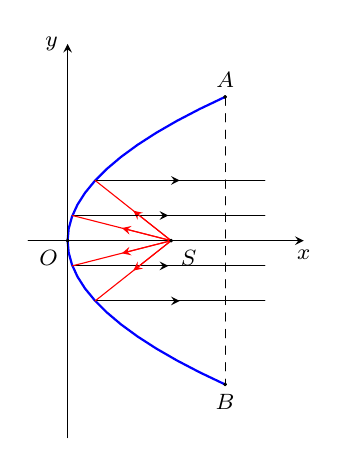
\begin{tikzpicture}[scale=0.5, font=\footnotesize, line join=round, line cap=round, >=stealth]

\draw[domain=-3.65:3.65, blue,thick] plot({3/10*(\x)^2},\x);
%\draw[gray!10] (-1,-1) grid (5,5);
\draw[->] (-1,0)--(6,0) node[below]{$x$};
\draw[->] (0,-5)--(0,5) node[left]{$y$};
\coordinate (A) at (4,3.65);
\coordinate (B) at (4,-3.65);
\coordinate (O) at (0,0);
\coordinate (C) at (0.12,0.64);
\coordinate (C') at (0.12,-0.64);
\coordinate (D) at (0.7,1.53);
\coordinate (D') at (0.7,-1.53);
\coordinate (F) at (5.01,1.53);
\coordinate (F') at (5.01,-1.53);
\coordinate (G) at (5.01,0.64);
\coordinate (G') at (5.01,-0.64);
\coordinate (E) at (2.63,0);
\coordinate (H1) at (1.67,0.76);
\coordinate (H2) at (1.67,-0.76);
\coordinate (H3) at (1.38,0.32);
\coordinate (H4) at (1.38,-0.32);
\coordinate (K1) at (2.85,1.53);
\coordinate (K2) at (2.85,-1.53);
\coordinate (K3) at (2.56,0.64);
\coordinate (K4) at (2.56,-0.64);
\draw  (F)--(D) (G)--(C) (F')--(D') (G')--(C') ;
\draw[dashed] (A)--(B);
\draw[red,->] (E)--(H1);
\draw[->] (D)--(K1) ;
\draw[red,->] (E)--(H3);
\draw[->] (C)--(K3) ;
\draw[red,->] (E)--(H4);
\draw[->] (C')--(K4) ;
\draw[red,->] (E)--(H2);
\draw[->] (D')--(K2) ;

\draw[red] (E)--(C) (E)--(D) (E)--(C') (E)--(D');

\draw[fill=black] (A) circle (1pt) node [above] {$A$};
\draw[fill=black] (B) circle (1pt) node [below] {$B$};
\draw[fill=black] (E) circle (1pt) node [below right] {$S$};
\draw[fill=black] (O) circle (1pt) node [below left] {$O$};
\end{tikzpicture}
}
\loigiai{
Từ giả thiết ta có parabol đi qua điểm $A(20;20)$ thay vào phương trình $y^2=2px$ do đó $20^2=2p\cdot 20\Leftrightarrow  p=10$.\\
Nên giá trị tham số tiêu là $p=10$.}
\end{ex}

\begin{ex}%[0H9V4-2]
	Trong mặt phẳng tọa độ $Oxy$, xét phương trình $x^2+y^2-2mx+2\left(m+1\right)y+5=0$ ($m$ là số thực). Có bao nhiêu giá trị nguyên của $m$ để phương trình đã cho là phương trình đường tròn có bán kính không vượt quá $2\sqrt{2}$.
	\par\shortans[oly]{$2$}
	\loigiai{
		Ta có $x^2+y^2-2mx+2\left(m+1\right)y+5=0$ \hfill (1).\\
		Phương trình $(1)$ là phương trình đường tròn khi và chỉ khi
		\begin{eqnarray*}
			&&m^2+\left(m+1\right)^2-5> 0\\
			&\Leftrightarrow& m^2+m-2> 0\\
			&\Leftrightarrow& \hoac{&{m > 1} \\&{m <-2}} \left(*\right).
		\end{eqnarray*}
		Khi đó đường tròn có bán kính $R=\sqrt{m^2+\left(m+1\right)^2-5}=\sqrt{2m^2+2m-4}$.\\
		Ta có $R\le 2\sqrt{2} \Leftrightarrow \sqrt{2m^2+2m-4} \le 2\sqrt{2} \Leftrightarrow m^2+m-6\le 0\Leftrightarrow-3\le m\le 2$.\\
		Kết hợp điều kiện $\left(*\right)$ ta được $m\in \left[-3;-2\right)\cup \left(1;2\right]$.\\
		Do $m\in \mathbb{Z}$ nên $m\in \left\{-3;2\right\}$. Vậy có $2$ giá trị nguyên $m$ thỏa mãn bài toán.
	}
\end{ex}

\Closesolutionfile{ans}

\TL
\begin{ex}
	Khai triển nhị thức $(1-3x^2)^5$.
\end{ex}


\begin{ex}%[0H9V4-2]%[Dự án đề kiểm tra Toán khối 10 HKI Năm 23-24-Dot15-Nguyễn Văn Sang]%[THPT Thieu Hoa- Thanh Hoá]
Trong mặt phẳng $Oxy$, cho đường tròn $(C)\colon x^2+y^2-2x-2y-23=0$ và điểm $M(7;3)$. 
\begin{enumerate}
	\item Viết phương trình đường tròn tâm $M$ và đi qua tâm đuờng tròn $(C)$.
	\item Lập phương trình đường thẳng $d$ qua $M$, cắt đường tròn tại  $2$  điểm $A$, $B$ sao cho $MA=3MB$.
\end{enumerate}
\loigiai{
\immini
{
Đường tròn $(C)$ có tâm $I(1;1)$ bán kính $R=5$, nhận thấy $M$ nằm ngoài hình tròn $(C)$.\\
Gọi $H$ là trung điểm $AB$ mà $MA=3MB \Rightarrow B$ là trung điểm $MH$.\\
Ta có $\heva{
& IH^2+MH^2=40 \\
& IH^2+BH^2=25 }\Leftrightarrow\heva{
& IH^2+4BH^2=40 \\
& IH^2+BH^2=25. }$\\
Suy ra $IH^2=20 \Rightarrow IH=2\sqrt{5}$.
}
{
\begin{tikzpicture}[line join = round, line cap = round,>=stealth,font=\footnotesize,scale=1]
\draw (0,0) circle (2cm);
\coordinate (A) at ($(0,0)+(-30:2cm)$);
\coordinate (B) at ($(0,0)+(-150:2cm)$);
\fill (0,0) circle (1pt) node[above]{$I$};
\fill (A) circle (1pt) node[right]{$A$};
\fill (B) circle (1pt) node[below]{$B$};
\coordinate (M) at ($(A)!3/2!(B)$);
\fill (M) circle (1pt) node[below]{$M$};
\coordinate (H) at ($(A)!1/2!(B)$);
\draw(M)--(A) (0,0)--(H) (M)--(0,0)--(B);
\fill (H) circle (1pt) node[below]{$H$};
\def\t{.15}\def\g{90}
\draw (H)--++(\g:\t)--++(0:\t)--++(-\g:\t);
\draw (A)--(H) node[midway] {$|$};
\draw (B)--(H) node[midway] {$|$};
\draw (B)--(M) node[midway] {$|$};
\end{tikzpicture}
}\noindent
Đường thẳng $d$ đi qua $M(7;3)$ có véc-tơ pháp tuyến $\overrightarrow{n}=(a;b)\neq \vec{0}$ có phương trình là \[a(x-7)+b(y-3)=0.\]
Ta có
\[
\begin{aligned}
& \mathrm{d}(I, d)=I H \\
& \Leftrightarrow \dfrac{|-6 a-2b|}{\sqrt{a^2+b^2}}=2 \sqrt{5} \\
& \Leftrightarrow 2 a^2+3 a b-2b^2=0 \\
& \Leftrightarrow 2\left(\dfrac{a}{b}\right)^2+3 \dfrac{a}{b}-2=0\\
& \Leftrightarrow \hoac{&\dfrac{a}{b}=\dfrac{1}{2} \\& \dfrac{a}{b}=-2.}
\end{aligned}
\]
\begin{itemize}
\item $\dfrac{a}{b}=\dfrac{1}{2} \Rightarrow a=\dfrac{b}{2} \Rightarrow(d)\colon x+2y-13=0$.
\item $a=-2b \Rightarrow(d)\colon 2x-y-11=0$.
\end{itemize}
}
\end{ex}

\begin{ex}%[0D0C2-6]%[Dự án đề kiểm tra Toán 10 HKII NH23-24- Trần Văn Hùng]%[THPT Nam Lý- Hà Nam]
	Cho đa giác đều có $15$ đỉnh. Gọi $M$ là tập tất cả các tam giác có ba đỉnh là ba đỉnh của đa giác đã cho. Chọn ngẫu nhiên một tam giác thuộc tập $M$. Tính xác suất để chọn được một tam giác cân nhưng không phải là tam giác đều.
	\loigiai{
	Số tam giác có ba đỉnh là ba đỉnh của đa giác đều $15$ cạnh là $\mathrm{C}_{15}^3=455$.\\
	Số phần tử không gian mẫu là $n(\Omega)=\mathrm{C}_{455}^1=455$.\\
	Gọi $A$ là biến cố \lq\lq Chọn được một tam giác cân nhưng không phải là tam giác đều\rq\rq\rq.
	\begin{itemize}
	\item Gọi $O$ là tâm đường tròn ngoại tiếp đa giác đều.
	\item Xét một đỉnh $A$ bất kì của đa giác đều: có $7$ cặp đỉnh của đa giác đối xứng với nhau qua $OA$, hay có $7$ tam giác cân tại đỉnh $A$.\\
	Như vậy, với mỗi đỉnh của đa giác có $7$ tam giác nhận nó làm đỉnh tam giác
	cân.
	\item Số tam giác đều có ba đỉnh là ba đỉnh của đa giác là $\dfrac{15}{3}=5$ tam giác.
	\item Tuy nhiên, trong các tam giác cân đã xác định ở trên có cả tam giác đều, do mọi tam giác đều thì đều cân tại ba đỉnh nên các tam giác đều được đếm ba
	lần.
	\item Suy ra số tam giác cân nhưng không phải tam giác đều có ba đỉnh là ba
	đỉnh của đa giác đã cho là $7\cdot 15-3\cdot 5=90$.
	\end{itemize}
	Xác suất của biến cố $A$ là $\mathrm{P}(A)=\dfrac{n(A)}{n(\Omega)}=\dfrac{90}{455}=\dfrac{18}{91}$.
	}
	\end{ex}
\Closesolutionfile{ansbook}

